\documentclass[a4paper, journal]{IEEEtran}
\IEEEoverridecommandlockouts
% The preceding line is only needed to identify funding in the first footnote. If that is unneeded, please comment it out.
\usepackage{cite}
\usepackage{amsmath,amssymb,amsfonts}
\usepackage{algpseudocode}
\usepackage{graphicx}
\usepackage{textcomp}
\usepackage{listings}
\usepackage{xcolor}
\usepackage{booktabs}
\usepackage{tikz}
\usepackage{times}
\usepackage{newtxmath}
\usepackage{algorithm}
\renewcommand{\ttdefault}{cmtt}
% \usepackage{courier}
% \usepackage[{cmtt}


\definecolor{codegreen}{rgb}{0,0.6,0}
\definecolor{codegray}{rgb}{0.2,0.2,0.2}
\definecolor{codepurple}{rgb}{0.58,0,0.82}
\definecolor{backcolour}{rgb}{0.95,0.95,0.92}

\lstset{
    language=Python,
    breaklines=true,
    breakatwhitespace=true,
    basicstyle=\ttfamily\footnotesize\color{codegray},
    keywordstyle=\color{codepurple}\bfseries,
    commentstyle=\color{codegreen}\itshape,
    stringstyle=\color{red},
    captionpos=b,
    frame=shadowbox,
    rulesepcolor=\color{gray},
    showstringspaces=false,
    tabsize=4,
    numbers=left,
    numberstyle=\tiny\color{codegray},
    stepnumber=1,
    numbersep=5pt,
    backgroundcolor=\color{backcolour},
    xleftmargin=15pt, % Add left margin
    xrightmargin=15pt % Add right margin
}


\hyphenation{op-tical net-works semi-conduc-tor IEEE-Xplore}
\def\BibTeX{{\rm B\kern-.05em{\sc i\kern-.025em b}\kern-.08em
    T\kern-.1667em\lower.7ex\hbox{E}\kern-.125emX}}
\usepackage{balance}
\begin{document}

\title{Maze Generation with Prim's Algorithm and Maze Solving with A* Search Algorithm}
\author{
    \IEEEauthorblockN{Dinanath Padhya\IEEEauthorrefmark{1}, Krishna Acharya\IEEEauthorrefmark{2}} \\
    \IEEEauthorblockA{\IEEEauthorrefmark{1}THA078BEI010 \quad \IEEEauthorrefmark{2}THA078BEI020\\
        Department of Electronics, Communication and Information Engineering\\
        Thapathali Campus, IOE, Tribhuvan University, Nepal\\
    }}

\maketitle




\begin{abstract}
    Maze generation and pathfinding are essential problems in the field of Artificial Intelligence, particularly in robotics, gaming, and autonomous navigation systems. In this lab, we implement a complete pipeline to generate and solve mazes using two classical algorithms. The maze is generated using a randomized version of Prim’s algorithm, which ensures the creation of a perfect maze, one with a unique solution and no cycles. Once generated, the maze is solved using the A* (A-Star) search algorithm, a widely used pathfinding technique that combines the benefits of uniform-cost search and heuristics to efficiently find optimal paths. We have developed Python-based implementations for both algorithms and used two visualization approaches, matplotlib for static/animated plotting and Pygame for interactive stepwise visualization. Finally, we analyze performance using metrics such as total nodes visited, total path length, and time taken for the solution, providing a comprehensive understanding of the search dynamics in generated mazes.
\end{abstract}

\section{Introduction}
Pathfinding and maze generation form the core of many artificial intelligence applications, including robotics, autonomous vehicles, and game development. Efficient generation and solving of mazes are crucial not only for entertainment but also for testing AI navigation capabilities under constrained environments.

This lab introduces two widely known algorithms in AI: Prim's algorithm for maze generation and the A* search algorithm for pathfinding. Prim's algorithm is a randomized, graph-based algorithm originally intended for finding minimum spanning trees, but with slight modifications, it can generate perfect mazes, mazes with no loops and a single solution path between any two points. This approach ensures that the maze has a structured yet unpredictable topology suitable for testing search algorithms.

Once the maze is constructed, we solve it using the A* algorithm, which is known for its optimal and complete nature when a consistent heuristic is used. A* operates using a best-first approach that balances the cost to reach a node (g-cost) and an estimated cost to the goal (h-cost), forming a total cost (f-cost = g + h). We use Manhattan distance as the heuristic due to the grid-based nature of the maze.

To enhance understanding and provide real-time feedback, we incorporated two visualization strategies: static/animated visualization using matplotlib and interactive visualization using Pygame. These help in observing the internal behavior of the search process and better interpret performance characteristics.

Through this lab, we aim to not only implement and compare these algorithms but also provide insight into their behavior, efficiency, and practical applications. The experiment reinforces core AI concepts such as heuristic search, graph traversal, and complexity trade-offs in algorithm design.



\section{Methodology}
This lab follows a structured pipeline that begins with maze generation using Prim’s algorithm, followed by the placement of start and goal positions. The generated maze is then solved using the A* search algorithm, and the entire process is visualized through both static/animated plots and an interactive GUI. Prim’s algorithm ensures the maze is a perfect maze, i.e., there is exactly one path between any two points. The A* algorithm efficiently finds the optimal path between the start and goal using a heuristic-based approach. For implementation, we used Python as the programming language along with libraries such as NumPy for numerical operations, matplotlib for plotting and animation, and Pygame for building an interactive visual interface.

\subsection{Maze Generation Using Prim’s Algorithm}

\subsubsection{Initialization}
We begin by initializing the maze as a 2D grid where all cells are set to walls (value 1). A random odd-indexed cell is chosen as the starting point and converted into a passage (value 0). This ensures that walls and passages are properly aligned in a grid with odd dimensions.

\subsubsection{Wall Selection and Carving}
From the starting cell, all adjacent walls (in four cardinal directions) are added to a frontier list. The algorithm proceeds by randomly selecting a wall from the frontier. If the cell on the opposite side of that wall is still a wall and has exactly one neighboring passage, the wall and the opposite cell are converted into passages. This process repeats until there are no more valid frontier walls.

\subsubsection{Properties}
This randomized wall-growing approach ensures that:
\begin{itemize}
    \item The resulting maze is \textbf{perfect} shown in Figure \ref{fig:maze_initial}, there exists a unique path between any two points with no loops.
    \item Each run of the algorithm produces a different maze structure due to random wall selection.
\end{itemize}

% \subsubsection{Algorithm}
\begin{algorithm}[H]
    \caption{Maze Generation using Prim’s Algorithm}
    \begin{algorithmic}[1]
        \Procedure{GenerateMaze}{rows, cols}
        \If{rows or cols even}
        \State Increment to make them odd
        \EndIf
        \State Initialize maze grid with all walls $(1)$
        \State Select random odd cell $(r, c)$ as start; set $maze[r][c] \gets 0$
        \State $walls \gets$ adjacent walls of $(r, c)$
        \While{$walls$ is not empty}
        \State Pick random wall $(r_1, c_1, r_2, c_2)$ from $walls$
        \If{$maze[r_2][c_2] = 1$ and only one adjacent cell to $(r_2, c_2)$ is a passage}
        \State $maze[(r_1 + r_2)/2][(c_1 + c_2)/2] \gets 0$ \Comment{Carve wall}
        \State $maze[r_2][c_2] \gets 0$
        \State Add new walls from $(r_2, c_2)$ to $walls$
        \EndIf
        \State Remove $(r_1, c_1, r_2, c_2)$ from $walls$
        \EndWhile
        \State \Return maze
        \EndProcedure
    \end{algorithmic}
\end{algorithm}

\begin{figure}
    \centering
    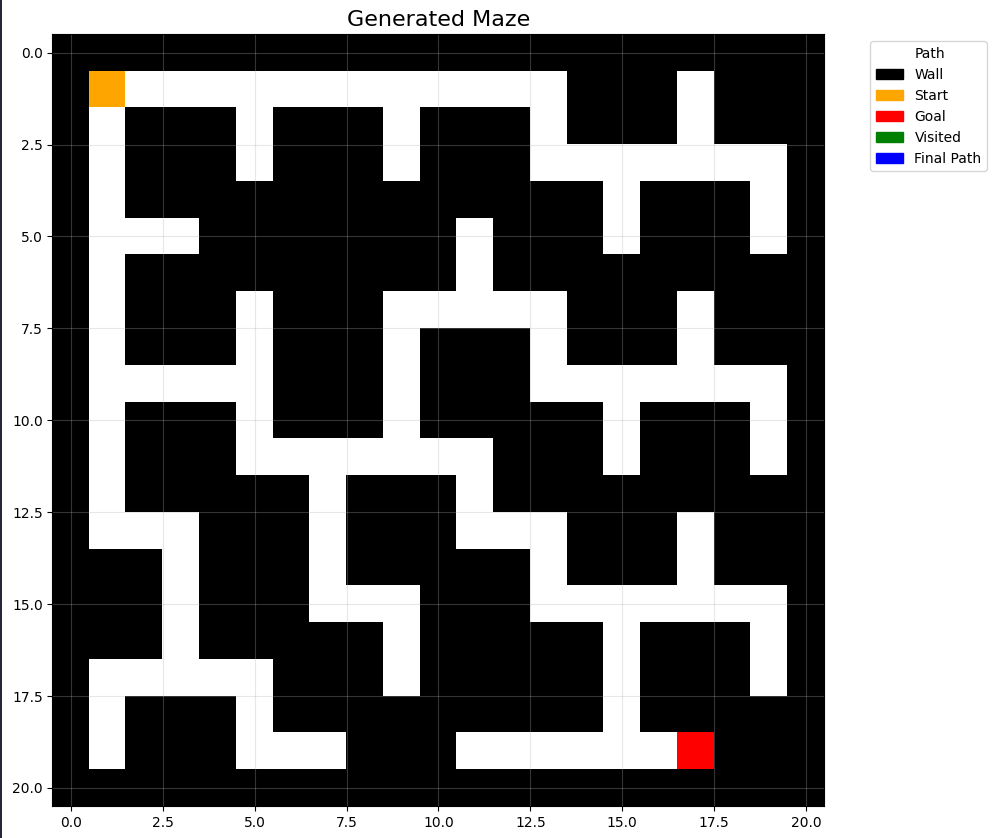
\includegraphics[width=0.5\textwidth]{./img/lab7/maze_initial.png}
    \caption{Initial Maze Generation using Prim's Algorithm}
    \label{fig:maze_initial}
\end{figure}


\subsection{Start and Goal Placement}

After generating the maze using Prim’s algorithm, we assign designated positions for the starting and goal points. According to the lab guidelines, the start point is placed at cell $(1, 1)$ and the goal point at cell $(rows - 2, cols - 2)$, both of which correspond to the first and last accessible inner positions of the maze grid.

To distinguish these points visually and programmatically, we encode them with unique integer values:
\begin{itemize}
    \item Start position $(1,1)$ is assigned the value \textbf{2}
    \item Goal position $(rows-2, cols-2)$ is assigned the value \textbf{3}
\end{itemize}

In the event that the default positions are blocked by walls, the algorithm searches for the next nearest valid passage cell in the respective direction (top-left for start, bottom-right for goal) and assigns the labels accordingly.

\vspace{0.5em}
\textbf{Function:} \texttt{place\_start\_goal(maze)}
The output maze looks like as in Figure \ref{fig:maze_initial}.

\vspace{0.5em}
\textbf{Returns:} A modified NumPy array with encoded start and goal positions.
\subsection{A* Search Algorithm Implementation}

\subsubsection{Cost Function}
The A* search algorithm uses a cost function to determine the most promising node to explore next:
\[
    f(n) = g(n) + h(n)
\]
where:
\begin{itemize}
    \item $g(n)$ is the actual cost from the start node to the current node $n$.
    \item $h(n)$ is the heuristic cost from node $n$ to the goal. In our implementation, this is computed using the Manhattan distance:
          \[
              h(n) = |x_{goal} - x_n| + |y_{goal} - y_n|
          \]
\end{itemize}

\subsubsection{Algorithm Steps}
The A* algorithm can be formally described as follows:

\begin{algorithm}[H]
    \caption{A* Search Algorithm}
    \begin{algorithmic}[1]
        \Procedure{AStarSearch}{maze, start, goal}
        \State Initialize open set as a priority queue containing start node with $f(start)$
        \State Initialize closed set as empty
        \While{open set is not empty}
        \State $current \gets$ node in open set with lowest $f$ value
        \If{$current = goal$}
        \State \Return reconstructed path from start to goal
        \EndIf
        \State Remove $current$ from open set
        \State Add $current$ to closed set
        \ForAll{neighboring nodes $n$ of $current$}
        \If{$n$ is a wall or $n$ in closed set}
        \State \textbf{continue}
        \EndIf
        \State $g_{tentative} \gets g(current) + 1$
        \If{$n$ not in open set or $g_{tentative} < g(n)$}
        \State Set parent of $n$ to $current$
        \State $g(n) \gets g_{tentative}$
        \State $h(n) \gets$ heuristic estimate to goal (e.g., Manhattan distance)
        \State $f(n) \gets g(n) + h(n)$
        \If{$n$ not in open set}
        \State Add $n$ to open set
        \EndIf
        \EndIf
        \EndFor
        \EndWhile
        \State \Return failure (no path found)
        \EndProcedure
    \end{algorithmic}
\end{algorithm}

The algorithm maintains two sets: an open set for nodes to be evaluated and a closed set for nodes already evaluated. It iteratively explores the most promising node based on the lowest $f$ value, expanding its neighbors and updating their costs until it finds the goal or exhausts all possibilities. Figure \ref{fig:maze_solved} illustrates the maze after applying the A* algorithm, showing the path from start to goal.

\begin{figure}
    \centering
    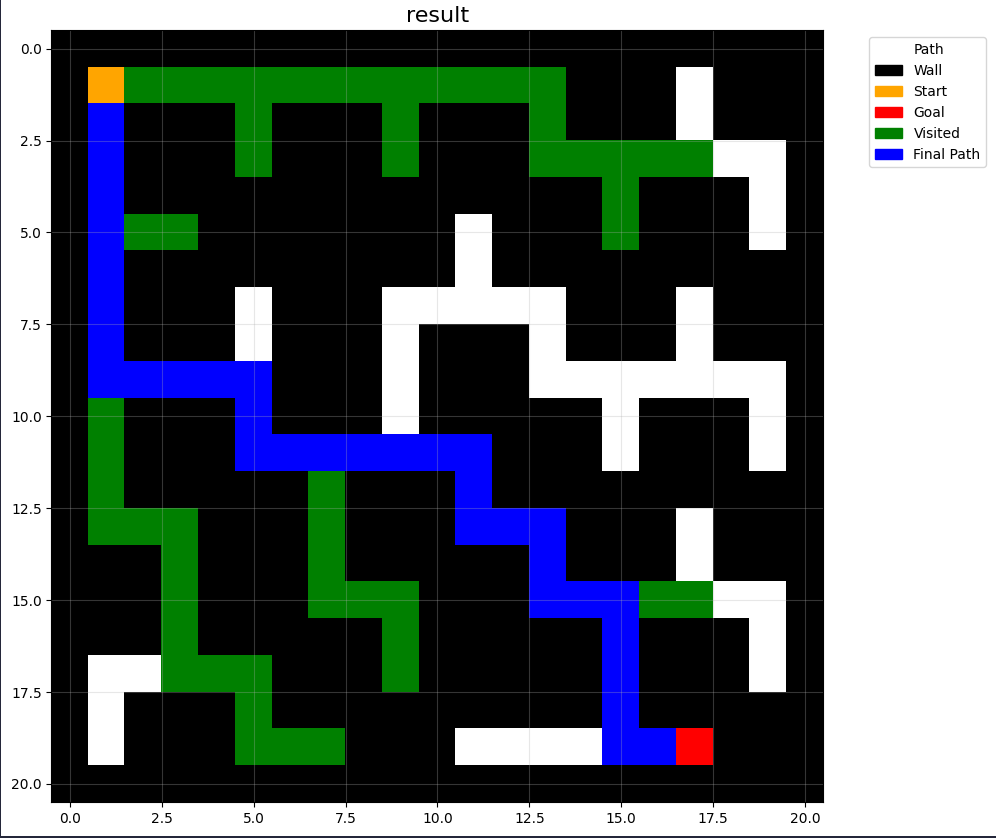
\includegraphics[width=0.5\textwidth]{./img/lab7/maze_solved.png}
    \caption{Maze Solved using A* Search Algorithm}
    \label{fig:maze_solved}
\end{figure}

\subsubsection{Metrics Recorded}
To analyze performance and efficiency, we record the following:
\begin{itemize}
    \item \textbf{Total nodes visited:} The count of all expanded/visited cells.
    \item \textbf{Path length:} The number of cells in the optimal path.
    \item \textbf{Execution time:} Total time taken to compute the solution path.
\end{itemize}

\begin{table}
    \caption{Performance Metrics}
    \centering
    \begin{tabular}{|c|c|c|c|}
        \hline
        \textbf{Maze Size} & \textbf{Total Nodes Visited} & \textbf{Path Length} & \textbf{Execution Time (s)} \\
        \hline
        20$\times$20       & 87                           & 35                   & 0.002                       \\
        10$\times$10       & 45                           & 15                   & 0.001                       \\
        \hline
    \end{tabular}
    \label{tab:results}
\end{table}

\subsection{Visualization Techniques}

\subsubsection{Matplotlib Static/Animated Visualization}
We used matplotlib to generate both static and animated visualizations of the maze-solving process. The maze is rendered with color coding for:
\begin{itemize}
    \item White – Passable path
    \item Black – Walls
    \item Orange – Start node
    \item Red – Goal node
    \item Green – Visited nodes
    \item Blue – Final solution path
\end{itemize}

\subsubsection{Pygame Interactive Interface}
For a more engaging and controlled experience, we developed an interactive GUI using Pygame as shown in Figure \ref{fig:pygame1}. The interface provides:
\begin{itemize}
    \item A ‘Start’ button to begin the solving animation.
    \item Real-time display of the current search node.
    \item Step-by-step progression through each search iteration.
    \item A final view highlighting the completed path from start to goal as shown in Figure \ref{fig:pygame2}.
\end{itemize}

\begin{figure}
    \centering
    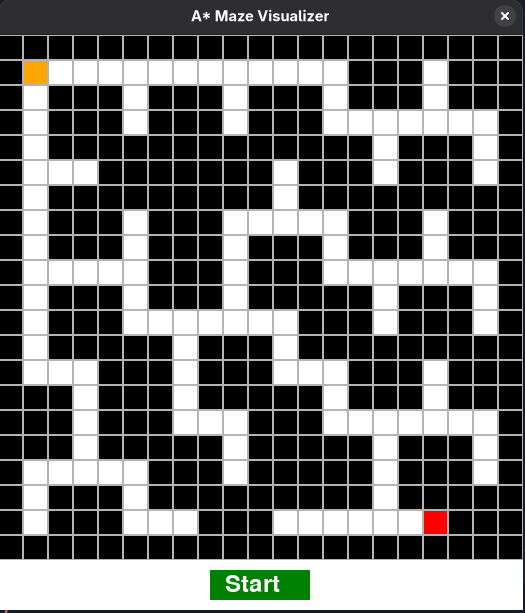
\includegraphics[width=0.4\textwidth]{./img/lab7/pygame1.png}
    \caption{Pygame Interactive Visualization of Maze Solving}
    \label{fig:pygame1}
\end{figure}

\begin{figure}
    \centering
    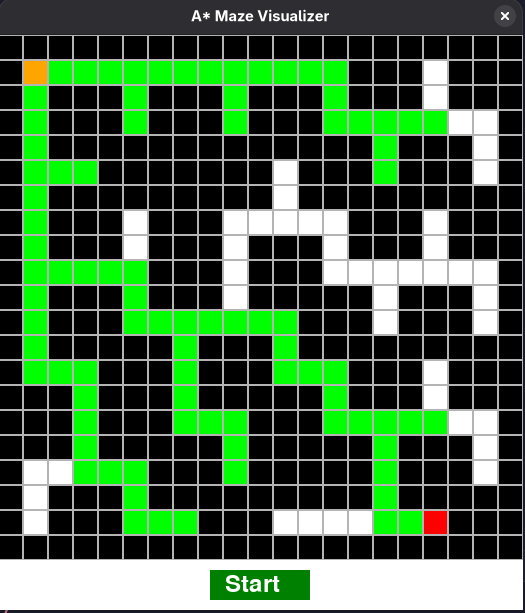
\includegraphics[width=0.4\textwidth]{./img/lab7/pygame2.png}
    \caption{Pygame Interactive Visualization of Maze Solving (Step-by-Step)}
    \label{fig:pygame2}
\end{figure}


\section{Results and Discussion}
The maze generation and solving process was successfully implemented, yielding various mazes and their respective solutions. The A* algorithm efficiently found paths in all generated mazes, demonstrating its effectiveness in grid-based pathfinding tasks.
The performance metrics collected during the experiments are summarized in Table \ref{tab:results}. The total nodes visited varied with maze complexity, while the path length remained consistent with the optimal solution characteristics of A*. The execution time was generally low, indicating the efficiency of the A* algorithm in this context.


\section{Conclusion}
This lab successfully demonstrated the generation of complex mazes and its efficient solution using A*. The heuristic-driven approach ensured optimal paths. The addition of Pygame visualization made the search process intuitive and engaging. Future enhancements may include support for DFS/BFS comparisons and weighted grid paths.


\bibliographystyle{IEEEtran}
\bibliography{ref}

\end{document}
